\documentclass[conference]{IEEEtran}
\usepackage{amsmath}
\usepackage{amssymb}
\usepackage{amsfonts}
\usepackage{graphicx}
\usepackage{float}
\usepackage[table]{xcolor}
\definecolor{forgetRed}{RGB}{255,200,200}
\definecolor{improveGreen}{RGB}{175, 225, 175}

\begin{document}

\title{[YOUR PAPER TITLE HERE]}
\author{\IEEEauthorblockN{[Your Name]}}
\maketitle

\begin{abstract}
Catastrophic forgetting remains a central challenge in continual reinforcement learning (CRL), where small shifts in task dynamics destabilize value estimates and degrade policy performance. Orthogonality-preserving regularization, such as Parseval networks, has been proposed to maintain representation stability, but its behaviour in classical control CRL settings is not well understood.
We evaluate Parseval-regularized Proximal Policy Optimization (Parseval PPO) on sequential variants of \texttt{CartPole-v1} and \texttt{Acrobot-v1}. We track critic geometry using layer-wise cosine similarity and relate these diagnostics to continual-learning metrics derived from a task--by--task evaluation matrix. On both benchmarks, Parseval PPO matches the episodic return of a standard PPO baseline and does not increase catastrophic forgetting. However, it maintains near-orthogonal critic layers while the baseline develops highly aligned representations. On Acrobot, we additionally observe that a task which is easy in isolation becomes harder mid-sequence, indicating that continual-learning difficulty can arise from representational interference rather than task complexity. Overall, Parseval regularization acts as a representation stabilizer in CRL, with geometric benefits that may become more important on larger or more challenging curricula.
\end{abstract}

\section{Introduction}

Continual reinforcement learning (CRL) aims to train agents that can solve a sequence of tasks without discarding previously acquired skills. In contrast to standard supervised continual learning, forgetting in RL is aggravated by non-stationary data, bootstrapped value targets, and policy-induced distribution shift. Policy-gradient methods such as Proximal Policy Optimization (PPO) are particularly brittle: moderate changes in dynamics can destabilize the critic, leading to noisy advantages and catastrophic forgetting even on relatively simple environments.

Recent work links such failures to \emph{representation collapse} in the critic, where weight matrices drift toward highly correlated and low-rank configurations. This reduces feature diversity, worsens value-function conditioning, and amplifies gradient variance, especially after task switches. As the critic becomes poorly conditioned, gradients fed into the policy become unreliable, so the agent may ``forget'' how to solve earlier tasks even if those tasks are still present in the environment distribution.

Orthogonality-based constraints, including Parseval regularization, address this problem by encouraging weight matrices to stay near-orthogonal, thereby controlling the Lipschitz constant and preserving diverse feature directions. Parseval networks were originally proposed for supervised learning and adversarial robustness, but the same mechanism---preventing features from collapsing onto a small number of correlated directions---is appealing for CRL, where new tasks continually place pressure on shared representations.

In this work we ask:

\begin{itemize}
    \item[RQ1] Does Parseval regularization improve learning performance across a sequence of tasks compared to standard PPO?
    \item[RQ2] Does it reduce catastrophic forgetting when tasks are presented sequentially with no replay or task IDs?
    \item[RQ3] Does it produce more stable and geometrically well-conditioned actor--critic representations during training?
\end{itemize}

We compare a standard PPO agent to a Parseval-regularized variant on sequential task variants of \texttt{CartPole-v1} and \texttt{Acrobot-v1}. For each environment, four physics configurations are presented sequentially. To study stability, we log layer-wise cosine similarity and relate these geometric measures to continual-learning metrics.

Our main findings are: (i) Parseval PPO attains similar returns and convergence speed to the baseline on both environments; (ii) catastrophic forgetting is limited on these small benchmarks for \emph{both} agents; (iii) Parseval PPO nevertheless keeps critic representations close to orthogonal, while the baseline exhibits strong feature alignment; and (iv) in Acrobot, a task that is easy when trained alone becomes substantially harder mid-sequence, highlighting how representational interference can create CRL difficulty even for simple tasks.

\section{Related Work}

\subsection{Continual Reinforcement Learning}

CRL methods aim to mitigate forgetting when agents encounter tasks sequentially. Approaches include replay buffers, regularization between tasks, knowledge distillation, and modular or multi-head architectures. Replay-based methods store past trajectories explicitly, whereas regularization approaches constrain parameter updates to remain close to previous solutions. Many benchmarks emphasise visual or replay-heavy settings, while classical control environments have received less attention despite being lightweight and interpretable. In particular, the role of the critic’s internal representation in driving forgetting and transfer in small control problems remains under-explored.

\subsection{Orthogonality and Parseval Regularization}

Orthogonality constraints have been used to stabilise training by preserving the norm of activations and preventing feature collapse. Parseval networks introduce a penalty that keeps $WW^\top$ close to a scaled identity, improving robustness and limiting the Lipschitz constant of each layer. Follow-up work extends orthogonality-preserving updates to deeper architectures and connects them to spectral regularisation and adversarial robustness. However, applications to RL and, specifically, continual RL are still rare. Our work examines whether such constraints improve critic geometry and forgetting behaviour in sequential control tasks, and whether geometric benefits can be observed even when returns remain similar.

\section{Method}

We compare a baseline PPO agent with a Parseval-regularized variant in two continual task sequences built from \texttt{CartPole-v1} and \texttt{Acrobot-v1}.

\subsection{PPO and Parseval-Regularized PPO}

The baseline agent uses clipped PPO with Generalized Advantage Estimation. The policy $\pi_\theta(a|s)$ and value function $V_\phi(s)$ are parameterised by two-layer MLPs of width 64 with \texttt{tanh} activations. Training follows a standard on-policy loop with mini-batch updates.

Parseval PPO augments the actor and critic losses with a Parseval penalty over each linear layer $W$:
\begin{equation}
    \mathcal{L}_{\text{parseval}}
    = \lambda \sum_W \big\| W W^\top - \alpha I \big\|_F^2,
\end{equation}
where $\alpha$ depends on the initialisation gain and $\lambda$ is a small coefficient. This term encourages rows of $W$ to remain approximately orthogonal. In some experiments we include diagonal scaling layers to preserve expressiveness while still controlling the effective Lipschitz constant. All other hyper-parameters (learning rate, batch size, clipping range) are matched between agents to isolate the effect of orthogonality.

\subsection{Sequential Task Setup}

For each environment we define four task variants by modifying physics parameters such as gravity, torque limits, masses, and link lengths. A \texttt{TaskManager} exposes these variants through a shared interface. Training proceeds through the sequence
\(
\mathcal{M}_1 \to \mathcal{M}_2 \to \mathcal{M}_3 \to \mathcal{M}_4
\),
with a switch every 300 episodes. Crucially, there is no replay buffer and no task identifier is appended to the state: from the agent's perspective, the environment simply drifts.

The network is never reset; the agent must adapt to new dynamics using the same parameters. After each 300-episode block we evaluate the current policy on all tasks for a fixed number of episodes, filling a task-by-task performance matrix $P \in \mathbb{R}^{T \times T}$, where $P_{t,i}$ is the mean return on task $t$ after finishing training on task $i$.

\subsection{Evaluation Metrics}

We report:

\begin{itemize}
    \item \textbf{Episodic return}: average return per episode during training, smoothed over a moving window. This shows how quickly each agent adapts to new tasks and whether performance collapses after switches.
    \item \textbf{Continual-learning metrics}: from $P$ we compute forward transfer (FWT), backward transfer (BWT), catastrophic forgetting (CF$=-$BWT), and a stability--plasticity balance $\text{SPB}=\text{FWT}-|\text{BWT}|$. These condense the matrix into scalar summaries of overall transfer behaviour.
    \item \textbf{Geometric diagnostics}: layer-wise cosine similarity between row vectors of the actor and critic weight matrices, focusing on the second hidden layer where collapse is most visible. Cosine values near~0 indicate diverse directions, whereas values near~1 indicate strong alignment.
\end{itemize}

All metrics are averaged over multiple seeds, and shaded regions in plots indicate 95\% confidence intervals across runs.

\section{Experiments and Results}
\label{sec:results}

We run both agents on CartPole-CL and Acrobot-CL, each comprising four tasks presented for 300 episodes each (2400 episodes total). Here we summarise the main observations; full curves appear in Figures~\ref{fig:cartpole_return_ci}–\ref{fig:acrobot_cosine_sim}.

\subsection{CartPole Continual Learning}

Figure~\ref{fig:cartpole_return_ci} shows episodic return on the CartPole sequence. Both agents rapidly reach high return on Task~1 and maintain strong performance across subsequent tasks. The mean curves nearly overlap and their 95\% confidence intervals remain strongly overlapping throughout training. Task switches create only shallow, short-lived dips, and both agents re-stabilise within a few dozen episodes.

\begin{table*}[t]
\centering
\caption{Mean Forgetting Across Environments (Base vs Parseval PPO)}
\setlength{\tabcolsep}{4pt}
\renewcommand{\arraystretch}{1.0}

\begin{tabular}{c|c|cc|cc|cc|cc}
\hline
\multirow{Environment} &
\multirow{Task} &
\multicolumn{2}{c|}{T1} &
\multicolumn{2}{c|}{T2} &
\multicolumn{2}{c|}{T3} &
\multicolumn{2}{c}{T4} \\
 & & Base & Parse & Base & Parse & Base & Parse & Base & Parse \\
\hline
\multirow{CartPole}
 & T1 & n/a & n/a
        & \cellcolor{improveGreen}-239.05 & \cellcolor{improveGreen}-231.91
        & \cellcolor{improveGreen}-311.30 & \cellcolor{improveGreen}-303.71
        & \cellcolor{improveGreen}-367.85 & \cellcolor{improveGreen}-384.36 \\
 & T2 & n/a & n/a & n/a & n/a
        & \cellcolor{improveGreen}-148.62 & \cellcolor{improveGreen}-117.82
        & \cellcolor{improveGreen}-227.96 & \cellcolor{improveGreen}-245.01 \\
 & T3 & n/a & n/a & n/a & n/a & n/a & n/a
        & \cellcolor{improveGreen}-74.81 & \cellcolor{improveGreen}-228.46 \\
 & T4 & n/a & n/a & n/a & n/a & n/a & n/a & n/a & n/a \\
\hline
\multirow{Acrobot}
 & T1 & n/a & n/a
        & \cellcolor{improveGreen}-58.37 & \cellcolor{improveGreen}-158.60
        & \cellcolor{improveGreen}-68.18 & \cellcolor{improveGreen}-161.52
        & \cellcolor{improveGreen}-66.33 & \cellcolor{improveGreen}-166.30 \\
 & T2 & n/a & n/a & n/a & n/a
        & \cellcolor{improveGreen}-3.77 & \cellcolor{improveGreen}-13.11
        & \cellcolor{improveGreen}-9.25 & \cellcolor{improveGreen}-16.70 \\
 & T3 & n/a & n/a & n/a & n/a & n/a & n/a
        & \cellcolor{improveGreen}-12.44 & \cellcolor{improveGreen}-5.81 \\
 & T4 & n/a & n/a & n/a & n/a & n/a & n/a & n/a & n/a \\
\hline
\end{tabular}
\end{table*}

\begin{table*}[t]
\centering
\caption{Performance Matrix (Mean Reward) Across Environments (Base vs Parseval PPO)}
\setlength{\tabcolsep}{6pt}
\renewcommand{\arraystretch}{1.05}

\begin{tabular}{c|c|c|cccc|cccc}
\hline
\multirow{Environment} &
\multirow{Episode} &
\multirow{Task} &
\multicolumn{4}{c|}{Base PPO} &
\multicolumn{4}{c}{Parseval PPO} \\
 & & & T1 & T2 & T3 & T4 & T1 & T2 & T3 & T4 \\
\hline
%%%%%%%%%%%%%%%%%%%%%%%%%%%%%%%%%%%%%%%%%%%%%%%%%%%%%%%%%%%%%%%%%%%%%%
\multirow{CartPole}
& 300  & T1 & 131.55 & 78.61 & 43.01 & 42.84
                & 79.86 & 49.25 & 39.88 & 36.43 \\
& 600  & T2 & 363.25 & 268.98 & 145.82 & 90.89
                & 330.35 & 207.71 & 100.74 & 64.52 \\
& 900  & T3 & 439.85 & 423.15 & 317.45 & 196.69
                & 375.80 & 319.41 & 166.12 & 105.44 \\
& 1200 & T4 & 500.00 & 499.48 & 411.89 & 293.54
                & 458.36 & 442.24 & 386.47 & 240.13 \\
\hline
%%%%%%%%%%%%%%%%%%%%%%%%%%%%%%%%%%%%%%%%%%%%%%%%%%%%%%%%%%%%%%%%%%%%%%
\multirow{Acrobot}
& 300  & T1 & -240.57 & -205.07  & -266.34 & -191.86
                & -310.85 & --178.60 & -342.34 & -267.47 \\
& 600  & T2 &  -183.13 & -150.99 & -198.65 & -132.08
                & -147.02 & -111.48 & -106.16 &-104.56 \\
& 900  & T3 & -179.46 & -143.76 & -210.56 & -133.04
                & -144.32 & -176.72 & -202.69 & -189.12 \\
& 1200 & T4 &  -178.60 & -140.31 & -203.20 & -125.93
                & -144.29 & -105.88 & -95.53 & -86.55 \\
\hline
\end{tabular}
\end{table*}


Continual-learning metrics on CartPole are correspondingly small: FWT and BWT are close to zero, CF is negligible, and SPB reflects that there is little trade-off between stability and plasticity on this easy benchmark. In terms of RQ1 and RQ2, Parseval regularisation neither substantially improves nor harms performance or forgetting on CartPole, but matches the baseline with statistically indistinguishable learning curves.

Acrobot is more challenging: returns are negative and closer to zero is better. As shown in Figure~\ref{fig:acrobot_return_ci}, both agents start with poor performance and gradually improve across tasks, with substantially wider confidence intervals than in CartPole. Variance between seeds is much higher, especially in the later cycles.

A notable phenomenon is that Task~3 becomes much harder in the continual sequence than in isolation. When trained alone, each Acrobot variant converges within roughly 300 episodes, but in the sequential regime both agents struggle to re-learn T3 after adapting to T1 and T2. This difficulty therefore reflects \emph{interference} from earlier tasks rather than intrinsic task complexity: the critic representation shaped by T1 and T2 does not align well with the value structure of T3, leading to unstable advantages and slow recovery.

Despite this, the two agents achieve comparable final performance on Acrobot, with overlapping CIs and no consistent winner. BWT is slightly positive on average, meaning that later training tends to slightly improve earlier tasks rather than degrade them. CF values are therefore near zero or negative, indicating that catastrophic forgetting is limited on this benchmark. From the perspective of RQ1 and RQ2, Parseval PPO behaves at least competitively with the baseline: it does not erase earlier knowledge and adapts to later tasks at a similar rate, even though Acrobot-CL is clearly more demanding than CartPole-CL.

\begin{figure}[t]
    \centering
    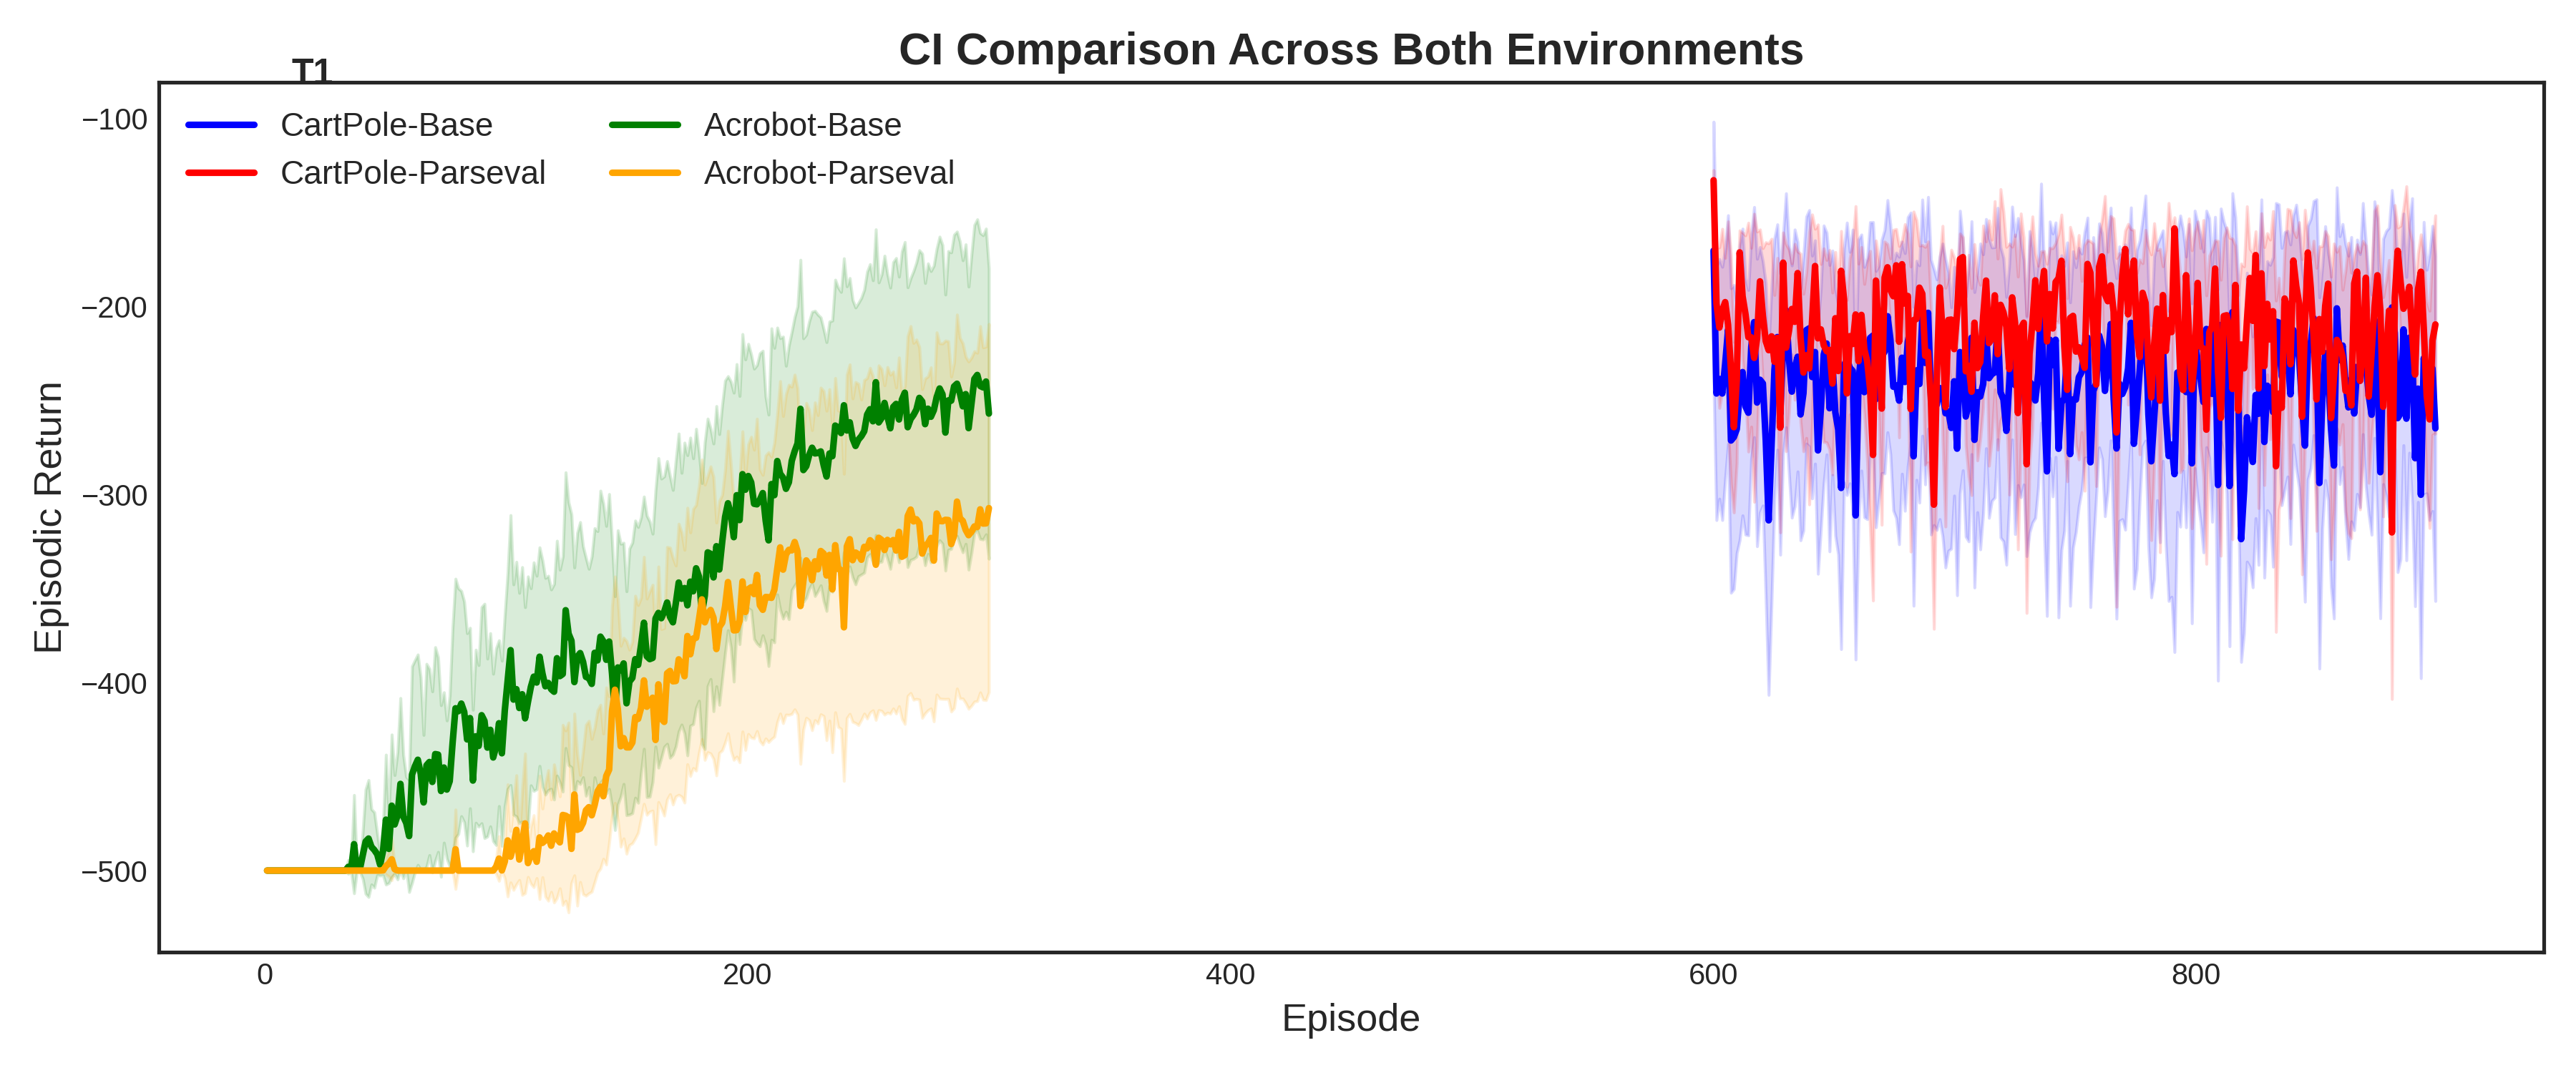
\includegraphics[width=\linewidth]{episodic_return.png}
    \caption{Episodic return on the Acrobot continual-learning sequence (95\% CI).}
    \label{fig:acrobot_return_ci}
\end{figure}

\subsection{Geometric Stability}

The clearest difference between the agents appears in their internal geometry. Figure~\ref{fig:acrobot_cosine_sim} plots the cosine similarity of the second hidden layer weights for the actor and critic on Acrobot-CL.

For the baseline PPO critic, cosine similarity increases steadily during training, indicating that weight vectors become increasingly aligned and the representation collapses toward a low-dimensional subspace. This behaviour is especially pronounced by the time the agent reaches Task~3, consistent with the observed difficulty in re-learning that task. The actor shows a similar, though slightly weaker, trend.

In contrast, the Parseval PPO critic maintains cosine similarity close to zero throughout training. Weight vectors remain approximately orthogonal, preserving a diverse feature basis. The same trend appears in the actor. This matches the intended effect of Parseval regularisation and echoes prior observations that orthogonality prevents feature collapse. Importantly, these differences are visible even though the return curves of the two agents are very similar, highlighting that geometric diagnostics can reveal changes in optimisation dynamics that are not obvious from performance alone.

These results answer RQ3: Parseval regularisation substantially stabilises actor--critic geometry, even though improvements in episodic return and CL metrics are modest on these small benchmarks.

\begin{figure}[t]
    \centering
    
\includegraphics[width=\linewidth]{critic_cosine_sim_layer_2.png}
    \caption{Layer-2 cosine similarity for actor and critic on Acrobot-CL. Lower values indicate more orthogonal features.}
    \label{fig:acrobot_cosine_sim}
\end{figure}

\section{Discussion and Limitations}

Across both environments, Parseval PPO achieves similar return and forgetting behaviour to standard PPO, but exhibits markedly more stable internal geometry. This suggests that on small control benchmarks, better conditioning of the critic does not automatically translate into higher sample efficiency, because PPO is already strong and catastrophic forgetting is limited.

The Acrobot experiments highlight a different failure mode: tasks that are easy in isolation can become hard mid-sequence due to representational interference. After adapting to Tasks~1 and~2, the critic’s feature space is specialised in a way that no longer matches the value landscape of Task~3, making re-learning unexpectedly slow. Parseval regularisation mitigates feature alignment but, in this setup, is not sufficient on its own to eliminate this effect. Combining orthogonality with other CRL mechanisms (e.g., replay or task-specific adapters) may be necessary for stronger gains.

Our study has several limitations. First, both environments are low-dimensional; they do not capture the rich observation spaces and severe interference patterns of realistic CRL applications. Second, the networks are shallow two-layer MLPs; orthogonality may matter more in deeper architectures where vanishing singular values are more severe. Third, the task sequence is short and task boundaries are known, whereas real deployments involve gradual and ambiguous shifts. Finally, we focus on cosine similarity and do not analyse other indicators of Lipschitz stability such as Jacobian norms or spectral concentration.

\section{Conclusion}

We investigated Parseval regularisation for PPO in continual reinforcement learning on CartPole-CL and Acrobot-CL. Parseval PPO matches the baseline in terms of episodic return and standard continual-learning metrics, and does not increase catastrophic forgetting. Its main effect is geometric: it keeps actor and critic weight matrices close to orthogonal and prevents the feature collapse observed in the baseline. The Acrobot sequence further shows that continual-learning difficulty can arise from representational interference even when individual tasks are easy. These findings support the view of Parseval regularisation as a representation stabiliser, and motivate future work on combining orthogonality constraints with more challenging CRL benchmarks, deeper networks, and additional mechanisms for mitigating interference.

% -----------------------------------------
% REFERENCES (put your .bib file name here)
% -----------------------------------------
\bibliographystyle{IEEEtran}
\bibliography{refs}  % <-- replace 'refs' with your .bib filename

\end{document}
